\chapter{Execução à nível de Programa}

  Esse capítulo apresenta as atividades e resultados obtidos na execução do processo a nível de Programa.
  
  \begin{figure}[!htbp]
    \centering
    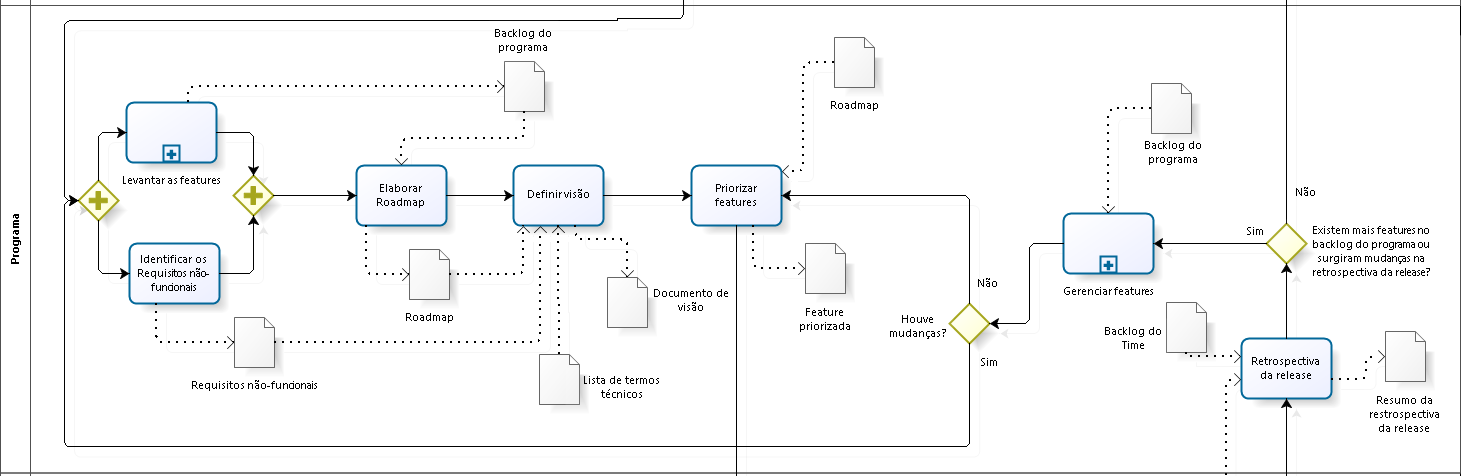
\includegraphics[scale=0.33]{figuras/processo_programa}
    \caption[Processo - Nível de Programa]{Processo - Nível de Programa.}
    \label{processo_programa}
  \end{figure}
  \vspace{0in}
  
  \section{Reuniões realizadas}
    
    A nível de programa foram realizadas duas reuniões com o cliente, que são brevemente resumidas nesta seção.
    
    \subsection{Resumo da 1ª reunião}
    
      No contexto do nível de Programa, a primeira reunião realizada utilizou a técnica de \textit{workshop}
      com \textit{brainstorming} para o levantamento das \textit{features} e dos requisitos não-funcionais da aplicação.
      A equipe de requisitos planejou o \textit{workshop} segundo a agenda apresentada na figura \ref{agenda_workshop}.
      
      \begin{figure}[!htbp]
	\centering
	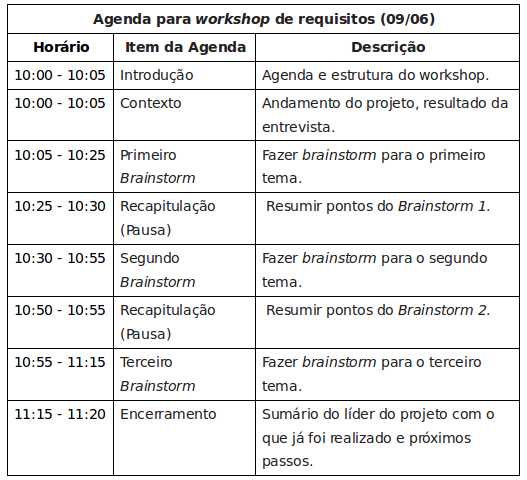
\includegraphics[scale=0.5]{figuras/agenda_workshop}
	\caption[\textit{Agenda do \textit{workshop} de requisitos} do projeto]{Agenda do \textit{workshop} de requisitos.}
	\label{agenda_workshop}
      \end{figure}
      
      Os temas dos \textit{brainstorms} eram, respectivamente, atividades da gestão operacional, atividades da gestão administrativa
      e questões referentes ao funcionamento e comportamento do sistema (requisitos não-funcionais). As ideias e colocações 
      geradas nos \textit{brainstorms} foram registradas em \textit{Post-its} pelos participantes do \textit{brainstorm}. 
      A figura \ref{post_its_reuniao} ilustra os resultados dos \textit{brainstorms} realizados.
      
      \begin{figure}[!htbp]
	\centering
	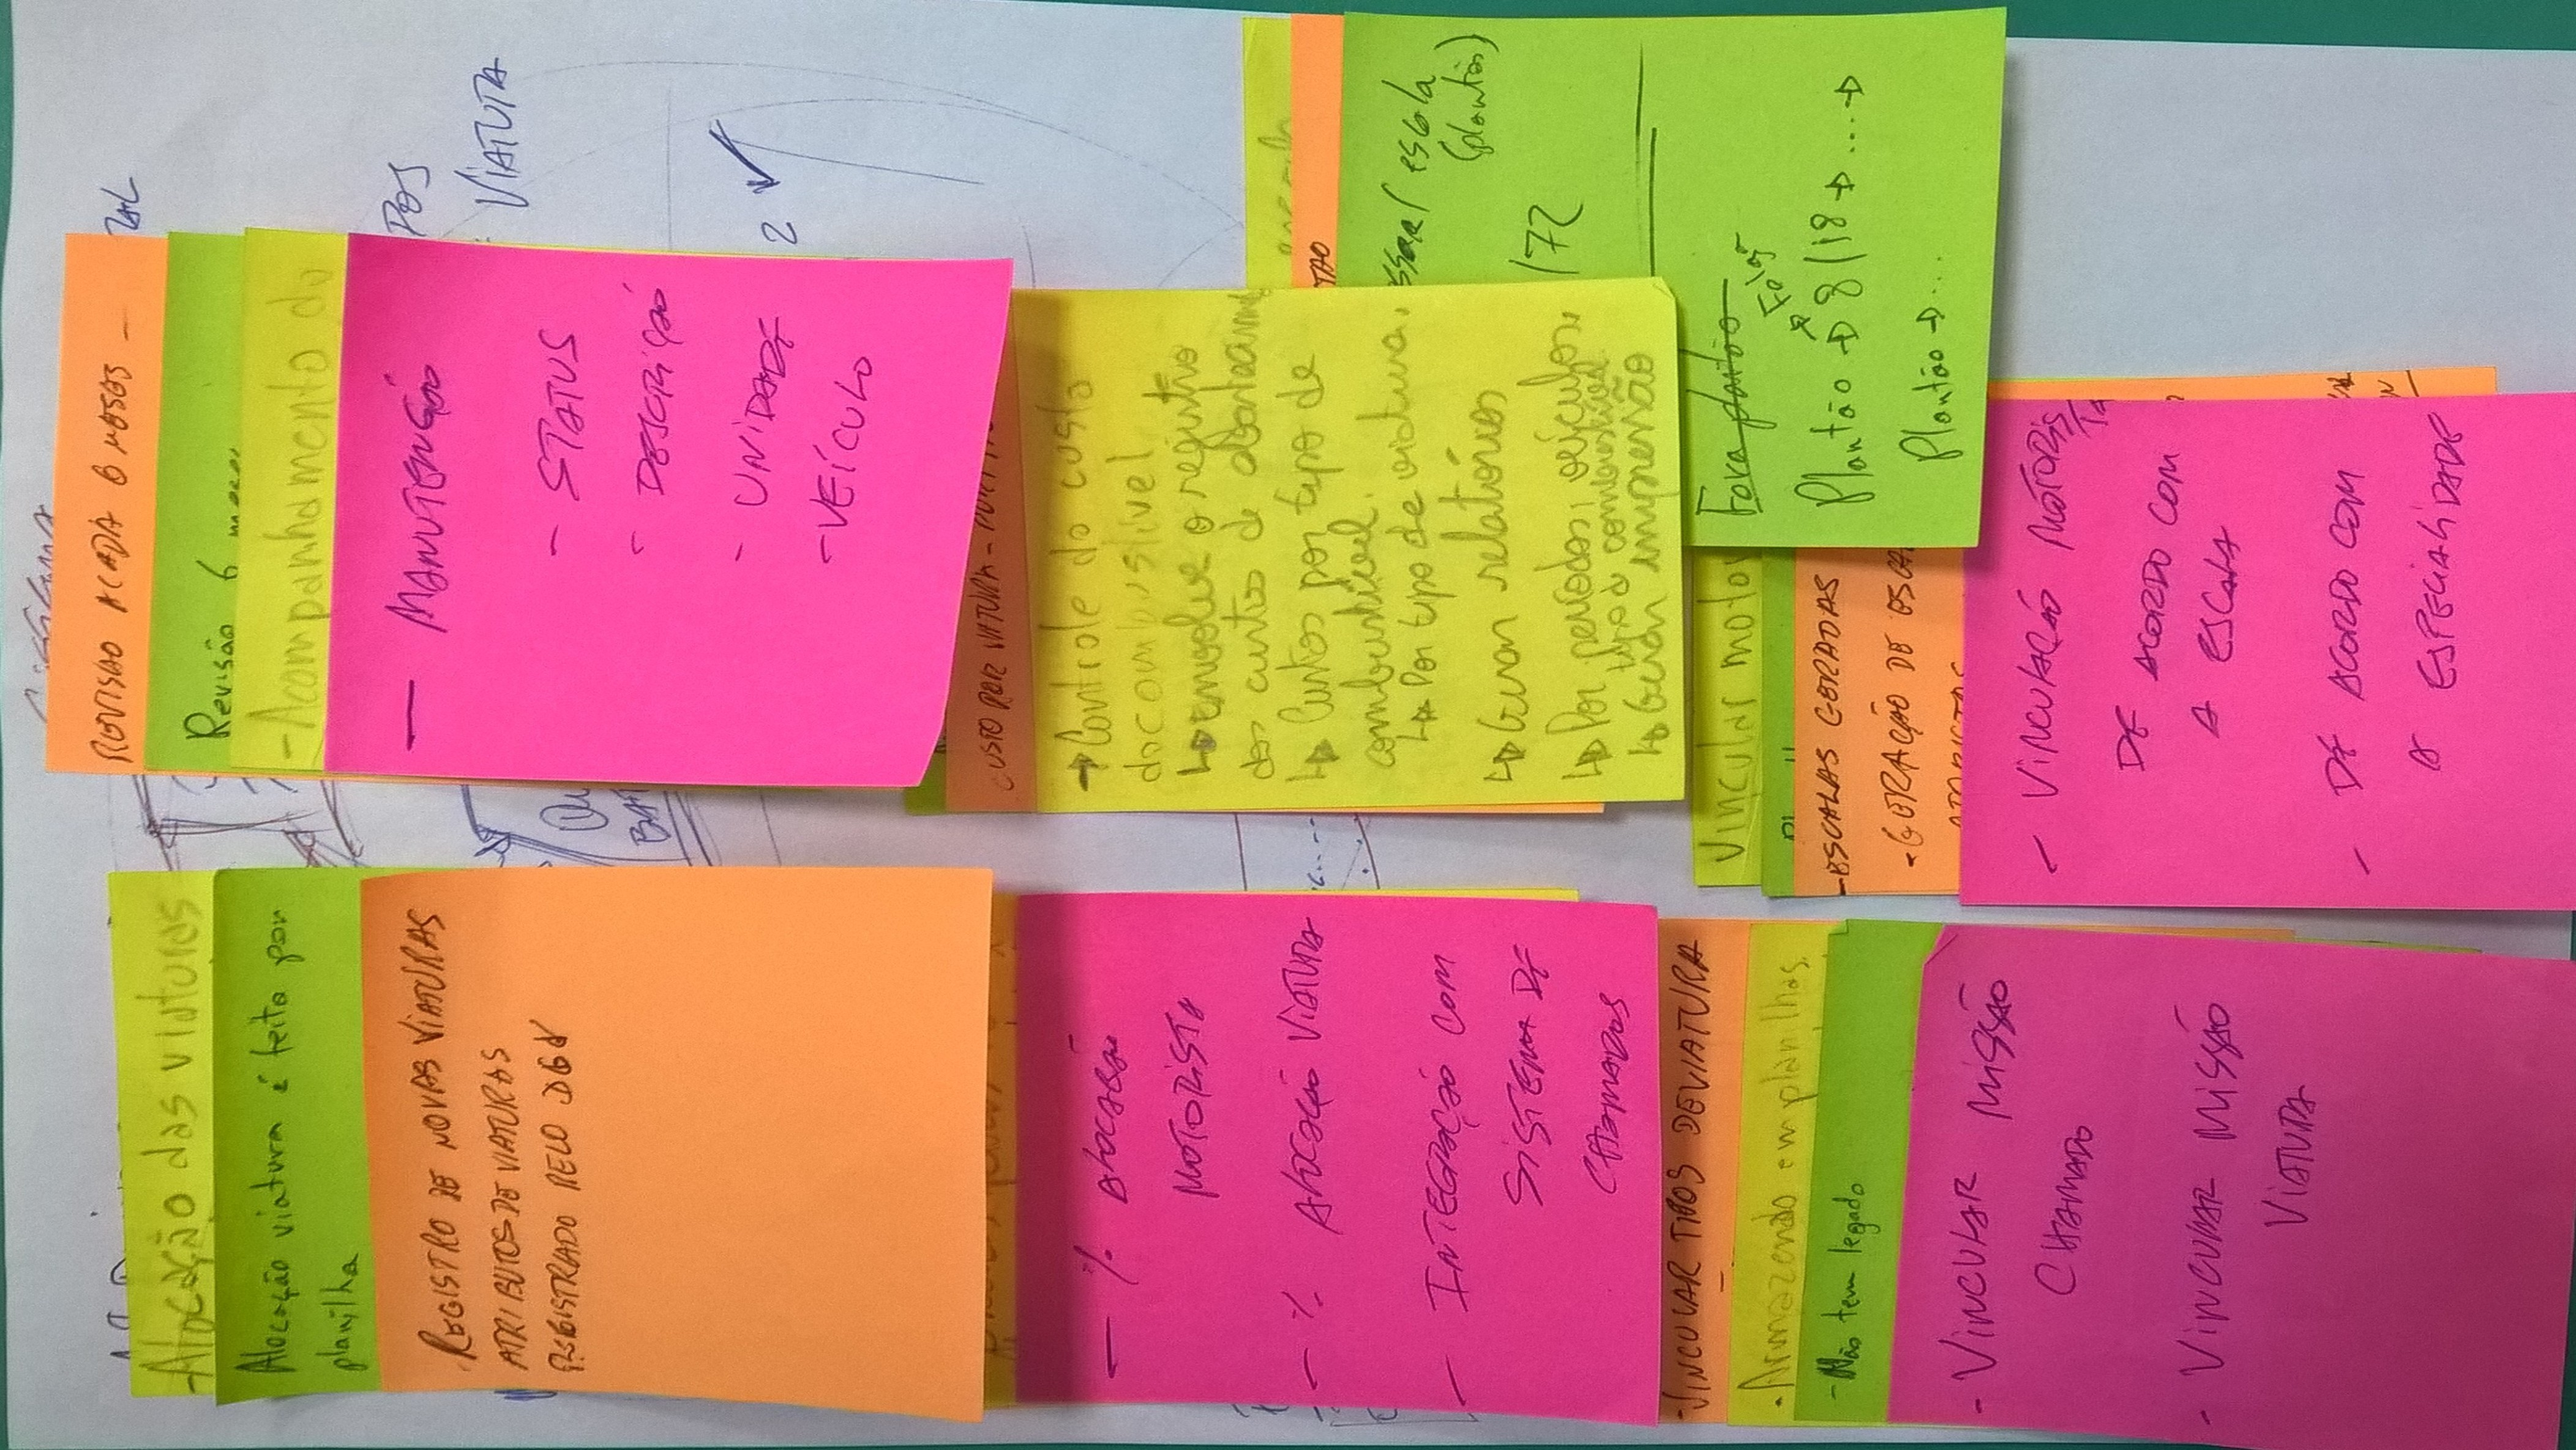
\includegraphics[scale=0.11]{figuras/post_its_reuniao}
	\caption[\textit{Post-its} com as colocações feitas no \textit{brainstorm}]
	  {\textit{Post-its} com as colocações feitas no \textit{brainstorm}.}
	\label{post_its_reuniao}
      \end{figure}
      
      Na prática, a reunião começou a nível de Portfólio quando foi validado com o cliente a priorização dos épicos
      (atividade de Priorizar épicos a nível de Portfólio). A partir dos épicos priorizados (segundo o cliente, os épicos tinham a 
      mesma relevância), conceitualmente, a reunião desceu para o nível de Programa com a realização dos \textit{brainstorms},
      realizando as atividades de "Levantar as \textit{features}" e "Identificar os requisitos não-funcionais" do nível de programa.
      
      Com o desenrolar da reunião, ainda foi possível levantar grande parte dos requisitos funcionais do sistema, embora este não tenha
      sido o objetivo inicial da reunião.
      
    \subsection{Resumo da 2ª reunião}
    
      Com as \textit{features} e os requisitos funcionais que foram identificados na reunião anterior, a equipe de requisitos 
      agrupou todas as ideias que já haviam sido levantadas e criou um mapa de conceitos (ilustrado na figura \ref{mapa_conceitos})
      para organizar os conceitos envolvidos no contexto e para identificar possíveis requisitos funcionais nas relações entre os 
      conceitos.
            
      \begin{figure}[!htbp]
	\centering
	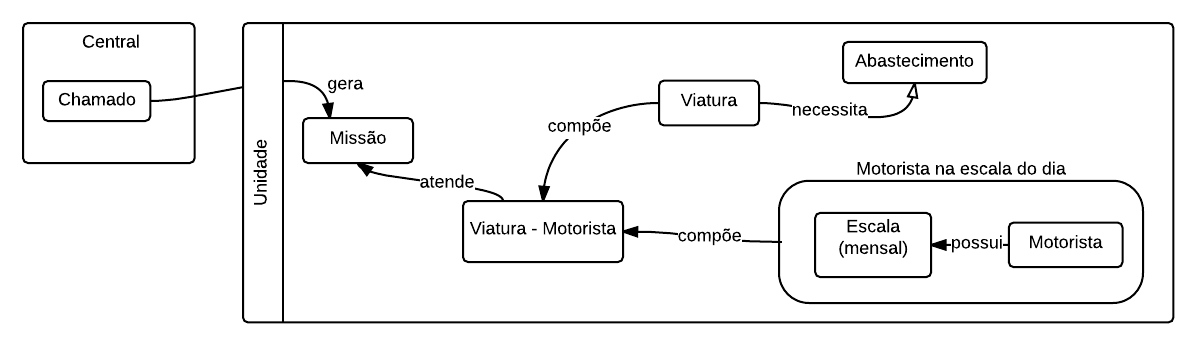
\includegraphics[scale=0.4]{figuras/mapa_conceitos}
	\caption[Mapa de conceitos para o contexto do sistema de gestão de viaturas]
	  {Mapa de conceitos para o contexto do sistema de gestão de viaturas.}
	\label{mapa_conceitos}
      \end{figure}
      
      Os requisitos funcionais identificados foram agrupados em casos de uso.
      O mapa de conceitos criado, juntamente com os requisitos identificados até o momento foi levado para o cliente para a
      validação do que foi produzido pela equipe.
      
      \subsubsection{Definição do escopo de implementação}
      
	Com a validação das \textit{features} definidas pela equipe ficou estabelecida a visão do projeto entre os
	\textit{stakeholders}. Com a visão estabelecida foi iniciada a construção do Documento de Visão e definido o
	escopo de implementação.
		
	Nessa reunião foi feita a validação inicial da priorização das \textit{features} no \textit{Roadmap} com o cliente. 
	Em conversa com o cliente, o \textit{Roadmap} precisaria apenas de algumas correções necessárias.
	
  
  \section{Considerações finais a nível de Programa}
    
    Esta seção apresenta um resumo dos itens mais importantes produzidos a nível de Portfólio.
    
    \subsection{\textit{Features} identificadas}
      
      O \textit{Backlog} do Programa ficou composto pelas seguintes \textit{features}:
      
      \begin{itemize}
       \item \textit{Feature} 1 (E1F1) - Gerenciamento das missões de unidade;
       \item \textit{Feature} 2 (E1F2) - Gerenciamento dos dados dos abastecimentos das viaturas;
       \item \textit{Feature} 3 (E1F3) - Consulta das viaturas das unidades por dispositivo móvel. 
       \item \textit{Feature} 4 (E2F4) - Gerenciamento dos motoristas da unidade;
       \item \textit{Feature} 5 (E2F5) - Gerenciamento das viaturas da unidade;
      \end{itemize}
      
      As \textit{features} estão descritas mais detalhadamente no documento de visão (apêndice \ref{doc_visao}).
              
    \subsection{Requisitos Não-funcionais}
    
          Os Requisitos não-funcionais consistem em restrições que o \textit{software} deve estar em conformidade ou qualidades específicas
          que o a solução deve ter. \cite{leffingwell14}
      
	  Para o levantamento dos requisitos não-funcionais foram analisados os conceitos do FURPS+ para a criação das perguntas que permitiram abstraí-los 
	  a partir de reuniões com o cliente.
	  
	  Os requisitos não-funcionais que foram levantados e validados com o cliente se encontram no Documento
	  de Visão (apêndice \ref{doc_visao}).
      
    \subsection{\textit{Roadmap}}
    
      
  De acordo com Leffingwell (\citeyear{leffingwell11}), o \textit{Roadmap} consiste numa série de \textit{releases} planejadas em datas, onde cada
  uma delas possui um tema e uma lista de \textit{features} priorizadas.
  
   \begin{figure}[!htbp]
    \centering
    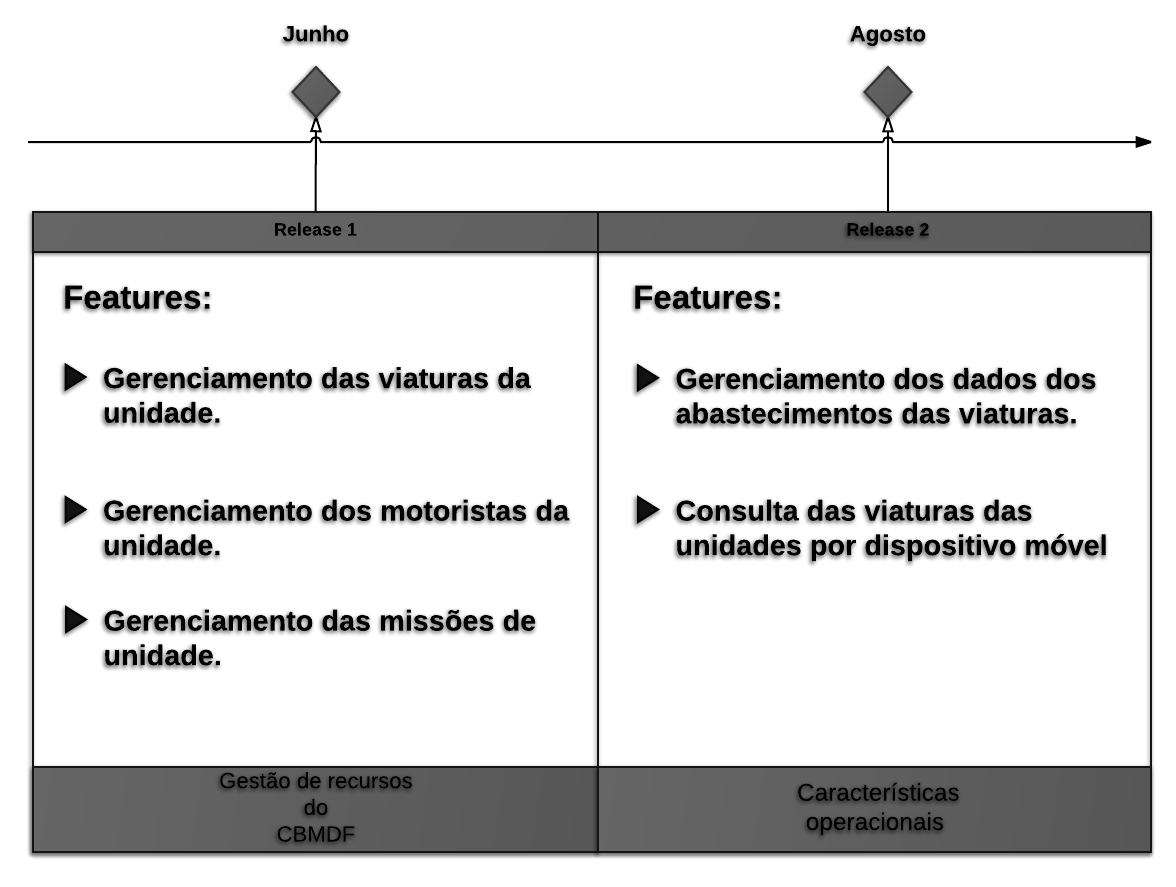
\includegraphics[scale=0.4, angle=0]{figuras/roadmap}
    \caption[\textit{Roadmap} do projeto.]{\textit{Roadmap} do projeto.}
    \label{fig:roadmap}
  \end{figure}
  
  Como ilustrado da Figura \ref{fig:roadmap}, o \textit{Roadmap} do projeto é composto por duas \textit{releases} com seus
  respectivos temas e datas. As \textit{features} foram alocadas e priorizadas, nas \textit{releases} a partir dos critérios: 
  
  \begin{itemize}
   \item Dependência funcional entre os requisitos;
    \subitem As \textit{features} estão alocadas em ordem de dependência funcional (de cima para baixo), bem como entre as
    \textit{releases} (da esquerda para direita).
    
   \item Importância relativa das mesmas para o cliente.
    \subitem As \textit{features} alocadas na \textit{release} 1 possuem maior importância e agregam maior valor ao cliente.
  \end{itemize}

    
    \subsection{Visão}
    
      O conteúdo primário da Visão de um sistema é o conjunto de features priorizadas que descrevem o que o sistema será capaz de oferecer 
      a seus usuários, para atender as necessidades dos envolvidos. \cite{leffingwell11}
      
      A visão do sistema acordada entre os \textit{stakeholders} encontra-se no documento de visão no apêndice \ref{doc_visao}
      
      \vfill
